\documentclass[a4paper,11pt]{article}
\usepackage[a4paper,margin=3.5cm]{geometry}
\usepackage{amsmath}
\usepackage{amssymb}
\usepackage{graphicx}
\usepackage[utf8]{inputenc}
\usepackage{polski}
\usepackage{hyperref}
\usepackage{float}

\title{Kosynteza systemów wbudowanych}
\author{P. Wlazły, T. Yerniyazov}
\date{Czerwiec 2024}

\begin{document}

\maketitle

\section{Opis}

Program zawiera implementację dwóch algorytmów stosowanych do kosyntezy systemów
wbudowanych:

\begin{enumerate}
    \item algorytm konstrukcyjny;
    \item przydział nieprzewidzianych zadań.
\end{enumerate}

\section{Algorytm konstrukcyjny}
Użytkownik podaje graf zadań oraz wartości maksymalnego dopuszczanego kosztu 
i czasu. Te dwie liczby mają istotny wpływ na przebieg całego algorytmu, gdyż
są stosowane podczas liczenia \ref{eq:pęd}.

\subsection{Kryterium wyboru}
Algorytm konstrukcyjny przydziela jednostki obliczeniowe poszczególnym 
zadaniom, stosując kryterium opierające się na znalezieniu wartości minimalnej z sumy trzech składowych standaryzowanych wcześniej do rozkładu 
o średniej równej 0 i odchyleniu standardowym równym 1:

\begin{equation}
    {Std}({x_i}) = \frac{x_i - \mu}{\sigma}
\end{equation}
\begin{itemize}
\item \(x_i\) - i-ta wartość,
\item \(\mu\) - średnia arytmetyczna wszystkich wartości,
\item \(\sigma\) - odchylenie standardowe.
\end{itemize}

Mając przygotowaną w postaci grafu zadań specyfikację systemy wbudowanego, wiemy,
jakie są koszt zakupu zasobu, koszt oraz czas wykonania na tym zasobie
rozważanego zadania. Nadając każdej z tych wartości określoną wagę, jesteśmy
w stanie sterować na bieżąco tym, jaki wpływ poszczególny parametr wywiera na
wybór typu jednostki obliczeniowej:

\begin{equation}
    L = min({w_1}\text{Std}(p) + {w_2}\text{Std}(c) + {w_3}\text{Std}(t))
    \label{eq:kryterium_wyboru}
\end{equation}
\begin{itemize}
\item \(w_i\) - i-ta waga,
\item \(p\) - koszt zakupu z tabeli @proc,
\item \(c\) - koszt wykonania zadania z tabeli @cost,
\item \(t\) - czas wykonania zadania z tabeli @times,
\item \text{Std}(•) - przekształcenie standaryzujące.
\end{itemize}

Po znalezieniu najlepszego zgodnie z zadanym kryterium typu zasobu są najpierw
sprawdzane jednostki obliczeniowe alokowane dotychczas. Jeżeli w spodziewanej
chwili rozpoczęcia zadania odpowiedni zasób zakupiony wcześniej jest wolny, to
zadanie jest wykonywane na tym zasobie. W przeciwnym razie, alokowany jest
dodatkowy zasób. Przy liczeniu czasu rozpoczęcia zadań uwzględniane są:
szyna danych łącząca zadanie z poprzednikiem; czas przesyłu określonej ilości
danych; sytuacja, w której zadanie może zostać wykonane na tym samym procesorze,
co poprzednie zadanie.

Trzeba zwrócić uwagę na to, że nowe zadania nie czekają na zwolnienie zasobów, a
zadania o potencjalnie krótszym czasie wykonania nie zawsze korzystają z
"okienek" pojawiających się w harmonogramach poszczególnych jednostek 
obliczeniowych. Dlatego proponujemy stosowanie naszego algorytmu do przygotowania punktu startowego algorytmów rafinacyjnych, które potrafią zoptymalizować początkowe rozwiązanie.


\subsection{Aktualizacja wag}
Współczynniki definiujące wagi do \ref{eq:kryterium_wyboru} są zmieniane
za pomocą podejścia opartego na pędzie obiektów fizycznych, czyli na wektorowej
wielkości opisującej mechanikę, a więc ruch i oddziaływania obiektów:

\begin{equation}
    \vec{p} = m \vec{v}
    \label{eq:pęd}
\end{equation}

gdzie:

\begin{equation*}
    m = 1 + \frac{n}{N}
\end{equation*}
\begin{itemize}
    \item \(n\) - liczba zadań, dla których dotychczas zostały zaalokowane
    zasoby (całkowita liczba zasobów do alokacji jest szacowana, bo jest szansa,
    że skorzystamy z zakupionych wcześniej zasobów),
    \item \(N\) - liczba wszystkich zadań;
\end{itemize}

\begin{equation*}
    \vec{v} = \frac{c}{C} - \frac{t}{T}
\end{equation*}
dla wartości z tabel @proc i @cost oraz:
\begin{equation*}
    \vec{v} = \frac{t}{T} - \frac{c}{C}
\end{equation*}
dla wartości z tabeli @times; Przy czym:
\begin{itemize}
    \item \(c\) - aktualna wartość kosztu systemu wbudowanego,
    \item \(C\) - maksymalny dopuszczalny koszt;
    \item \(t\) - aktualna wartość czasu wykonania (czas zakończenia zadania,
    które ma zasób i zostanie wykonane najpóźniej),
    \item \(T\) - maksymalny dopuszczalny czas;
\end{itemize}

Dzięki temu, że wektor prędkości \(\vec{v}\) ma inny zwrot przy liczeniu wag
do kosztów i wagi do czasu wykonania, jesteśmy w stanie zwiększać bądź zmniejszać
wpływ każdego z tych czynników. Ponadto, analogia do masy obiektu pozwala na
zmianę tego, jak mocno wektory pędu przesuwają współczynniki do przodu bądź do
tyłu w przestrzeni jednowymiarowej: jeżeli jesteśmy dopiero na samym początku 
procesu alokowania zasobów i przed nami jest jeszcze duża liczba \(N\) zadań, to
aktualizacja wag będzie dosyć wolna. Zbliżając się do momentu, kiedy zostaje
coraz mniej zadań do załatwienia, chcemy przyspieszyć proces aktualizacji 
współczynników \(w_i\), gdyż pamiętamy o ograniczeniach czasowych i finansowych
podanych przez użytkownika podczas uruchomienia programu.

Żeby zapobiec potencjalnej niestabilności numerycznej wynikającej ze zmiany
wag przez długi okres w przypadku dużych grafów zadań, postanowiliśmy
stosować normalizację przesuniętych współczynników do prawdopodobieństwa za
pomocą funkcji Softmax:

\begin{equation}
    \text{Softmax}(x_i) = \frac{e^{x_i}}{\sum_{j=1}^{3} e^{x_j}}
\end{equation}

Dzięki temu wagi inicjalizowane pierwotnie jako \(\frac{1}{3}\) zawsze 
mieszczą się w zakresie od 0 do 1 (stąd też dodanie 1.0 do masy, bo
mnożenie ułamków tłumiłoby cały postęp).

\subsection{Skuteczność}
Sprawdziliśmy na dużym grafie testowym (200 zadań), jakie wyniki otrzymujemy 
dla różnych wartości maksymalnego czasu i kosztu. Zachowanie algorytmu przy
ustalonym koszcie maksymalnym, ale zmiennym czasie maksymalnym, widoczne jest
na wykresie \ref{fig:plot_1}. Odwrotne podejście (zmienialiśmy wartość maksymalnego dopuszczalnego kosztu, mając ustalony maksymalny czas) daje zachowanie przedstawione na wykresie \ref{fig:plot_2}.

\begin{figure}[H]
    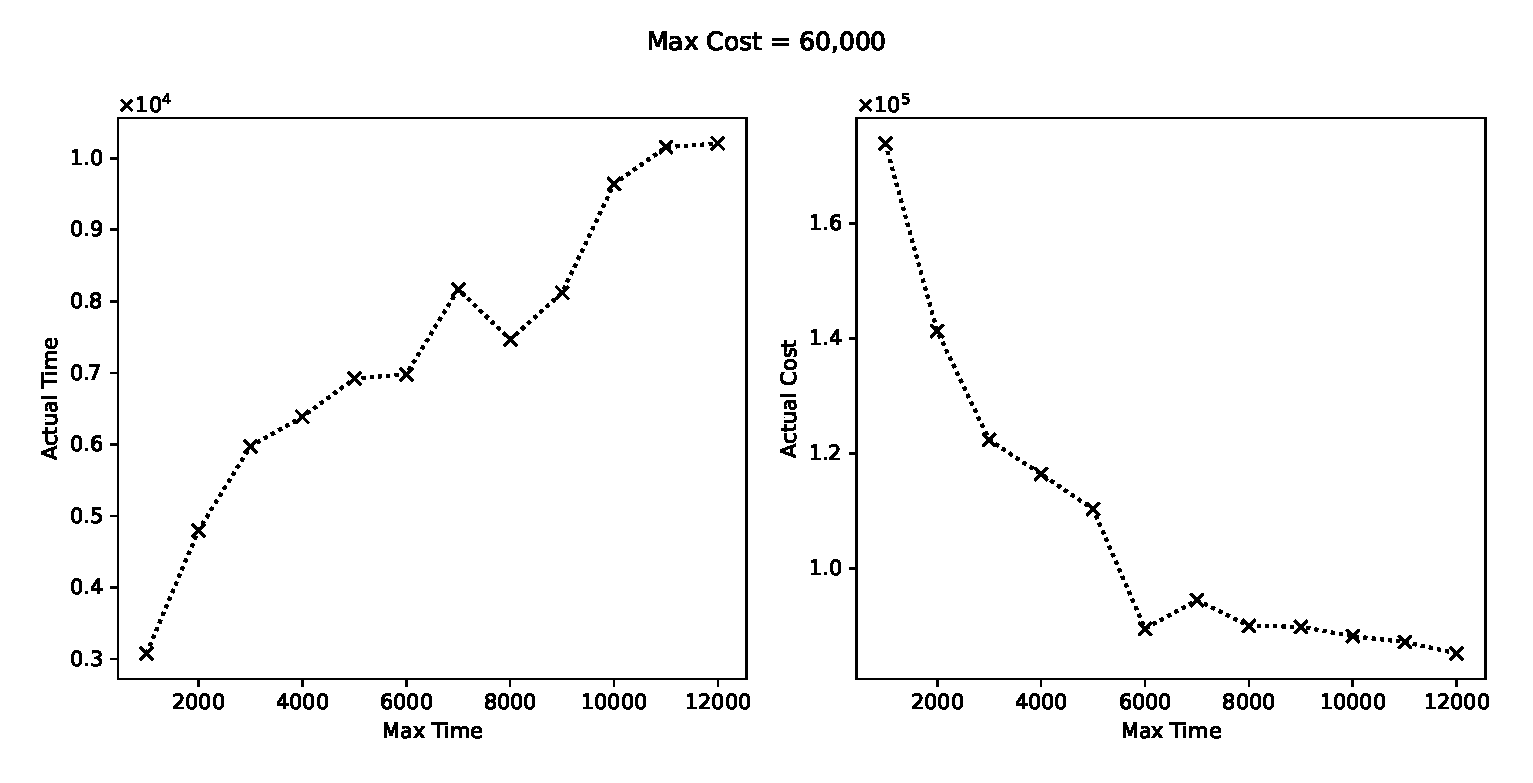
\includegraphics[width=\textwidth]{Figure_1.eps}
    \caption{Obserwacja zmiany całkowitego kosztu i czasu systemu wbudowanego przy różnych wartościach maksymalnego czasu i stałej wartości maksymalnego dopuszczalnego kosztu (\(c_{max}=60000\)).}
    \label{fig:plot_1}
\end{figure}

\begin{figure}[H]
    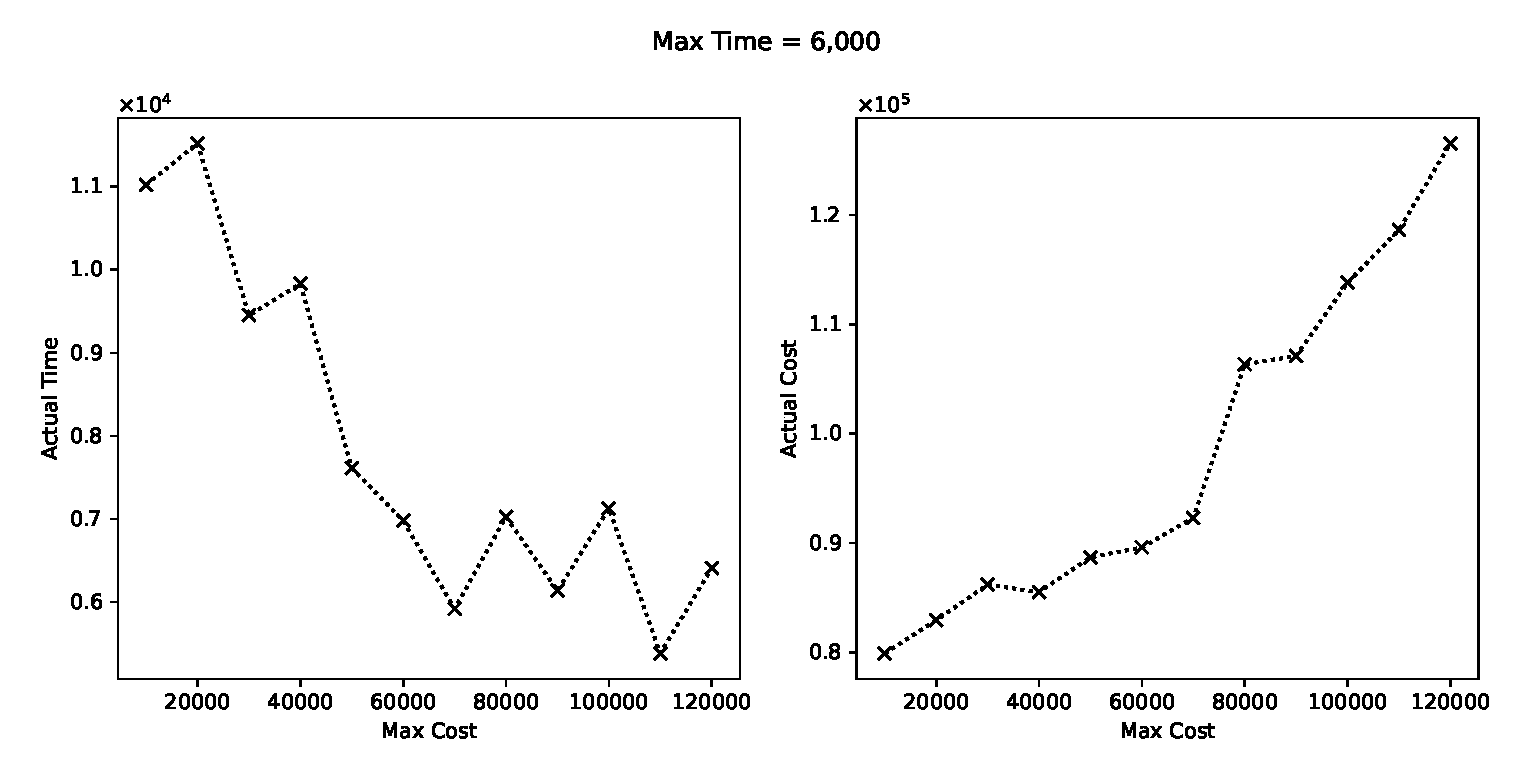
\includegraphics[width=\textwidth]{Figure_2.eps}
    \caption{Obserwacja zmiany całkowitego kosztu i czasu systemu wbudowanego przy różnych wartościach maksymalnego kosztu i stałej wartości maksymalnego dopuszczalnego czasu (\(t_{max}=6000\)).}
    \label{fig:plot_2}
\end{figure}

Poniżej załączony jest wynik uruchomienia innego grafu, który zawierał 10
zadań. Podano w tym przypadku parametry \(t_{max}=1000\) i \(c_{max}=600\).

\begin{verbatim}
Alokacja zasobów metodą standaryzacji:
  T0 --> HC1_0 [startTime: 0, endTime: 15]
  T1 --> HC1_1 [startTime: 18.8, endTime: 36.8]
  T2 --> PP1_0 [startTime: 45.8, endTime: 240.8]
  T3 --> PP1_1 [startTime: 47.6, endTime: 182.6]
  T4 --> HC1_1 [startTime: 246, endTime: 257]
  T5 --> PP1_2 [startTime: 194.4, endTime: 231.4]
  T6 --> HC1_0 [startTime: 244.8, endTime: 261.8]
  T7 --> PP1_3 [startTime: 189.8, endTime: 462.8]
  T8 --> PP1_2 [startTime: 250.6, endTime: 318.6]
  T9 --> HC1_1 [startTime: 272.6, endTime: 290.6]

Całkowity czas wykonania: 462.8
Całkowity koszt: 7855    
\end{verbatim}

Widać, że przekroczony został maksymalny koszt, co jest dozwolone 
w naszej implementacji algorytmu konstrukcyjnego.

\section{Przydział nieprzewidzianych zadań}

Program wczytuje dane z grafu zadań zawierającego nieprzewidziane zadania
oznaczone jako "uT" (z ang. \textit{unexpected task}). Następnie przydzielane 
są zasoby do każdego zadania, przy czym nieprzewidziane zadania mają dostęp
wyłącznie do zasobów uniwersalnych. Stosowane kryterium to:

\begin{equation}
    L = min(t \times c)
\end{equation}
\begin{itemize}
\item \(t\) - wartość z tabeli @times,
\item \(c\) - wartość z tabeli @cost.
\end{itemize}

Zakładamy, że posiadamy po jednej kopii każdego typu zasobu, 
w związku z czym kolejny krok polega na dokonaniu szeregowania listowego, 
obliczając ścieżki krytyczne. Przydział nieprzewidzianych zadań nie uwzględnia
szyn komunikacyjnych, ponieważ nie wiemy, jak postąpić w sytuacji, kiedy
przewidziane zadania nie mogą zostać wykonane na dostępnych zasobach ze względu
na brak połączeń między tymi, co jest możliwe po usunięciu z listy zasobów 
jednostek specjalistycznych. 
\\\\
Wynik uruchomienia programu na przykładowym grafie wygląda następująco:

\begin{verbatim}
Początkowy przydział zasobów
  T0 --> HC1
  T1 --> HC1
  T2 --> HC1
  T3 --> HC1
  T4 --> HC1
  T5 --> HC1
  T6 --> HC1
  T7 --> HC1
  T8 --> HC1
  T9 --> HC1
  uT10 --> PP1
  uT11 --> PP2
  uT12 --> PP1
  uT13 --> PP2

Poszeregowane zadania (w tym nieprzewidziane):
  T0 --> T1 --> T2 --> T3 --> T7 --> uT11 --> T4 --> T5 --> T8 
  --> uT10 --> uT13 --> uT12 --> T6 --> T9
\end{verbatim}

\section{Podsumowanie}
W niniejszym dokumencie przedstawiono różne od siebie problemy kosyntezy systemów 
wbudowanych oraz opisano metody ich rozwiązania: algorytm konstrukcyjny i algorytm 
przydziału nieprzewidzianych zadań. Podczas implementacji obu algorytmów napotkano 
szereg wyzwań, z którymi należało się zmierzyć. Pierwszym z nich było zaprojektowanie 
kryterium wyboru optymalnego typu zasobu dla każdego zadania. Wymagało to 
uwzględnienia wielu czynników, takich jak koszt zakupu, koszt wykonania oraz 
czas wykonania zadania. Ponadto, konieczne było odpowiednie skalowanie tych 
czynników poprzez nadanie im odpowiednich wag oraz zapewnienie, aby wpływ każdego 
czynnika na ostateczny wybór był odpowiednio zrównoważony. Kolejnym wyzwaniem 
było efektywne zarządzanie zasobami podczas przydziału nieprzewidzianych zadań. 
Konieczne było skonstruowanie algorytmu, który uwzględniał minimalny iloczyn 
czasu i kosztu, jednocześnie zapewniając, że zadania te były wykonywane w sposób 
zbliżony do optymalnego i w miarę zminimalizowany kosztowo. W rezultacie, oba 
algorytmy zostały zaimplementowane i przetestowane na przykładowych danych, 
demonstrując swoją skuteczność. Pomimo napotkanych trudności, uzyskane wyniki 
stanowią niezłą podstawę do dalszych badań i ewentualnych udoskonaleń algorytmów 
w przyszłości.


\end{document}